\chapter{Upload and manage images}

A virtual machine \gls{OpenStack Image}, referred to in this document simply as an
image, is a single file that contains a virtual disk that has a bootable
operating system installed on it. Images are used to create virtual
machine instances within the cloud. For information about creating image
files, see the
\href{https://docs.openstack.org/image-guide/}{\emph{OpenStack Virtual
Machine Image Guide}}.

Depending on your role, you may have permission to upload and manage
virtual machine images. Operators might restrict the upload and
management of images to cloud administrators or operators only. If you
have the appropriate privileges, you can use the dashboard to upload and
manage images in the admin project.

~

Note

You can also use the \textbf{openstack} and \textbf{glance} command-line
clients or the Image service to manage images.

\strong{Upload an image}

Follow this procedure to upload an image to a project:

\begin{enumerate}
\def\labelenumi{\arabic{enumi}.}
\item
  \begin{quote}
  Log in to the dashboard.
  \end{quote}
\item
  \begin{quote}
  Select the appropriate project from the drop down menu at the top
  left.
  \end{quote}
\item
  \begin{quote}
  On the Project tab, open the Compute tab and click Images category.
  \end{quote}
\item
  \begin{quote}
  Click Create Image.
  \end{quote}
\end{enumerate}

\begin{quote}
The Create An Image dialog box appears.

\begin{center}
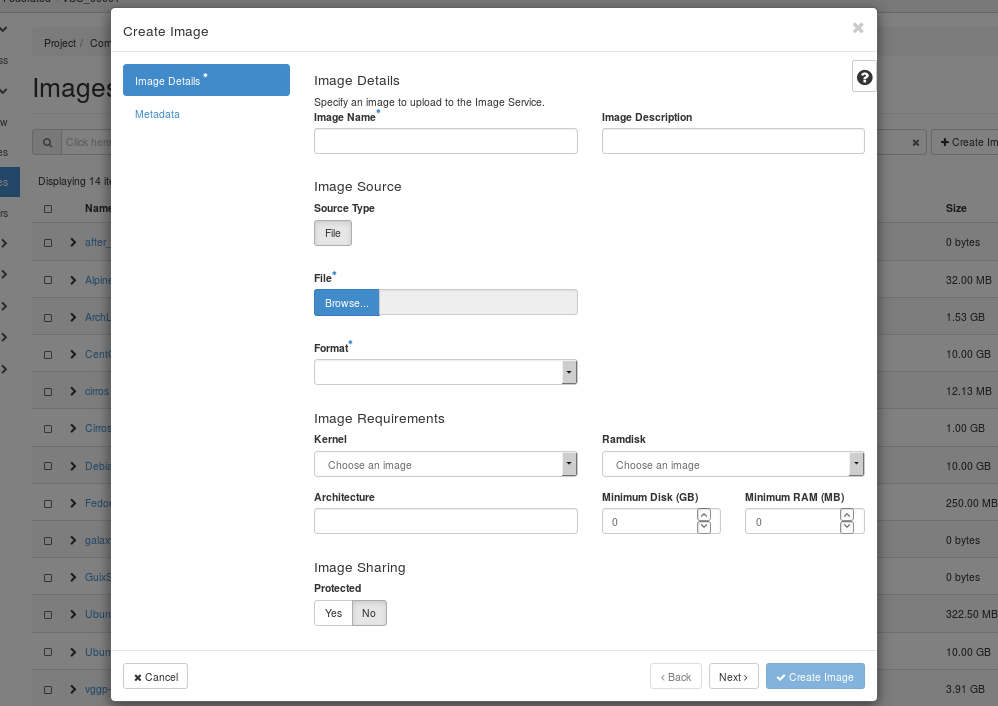
\includegraphics[scale=0.4]{img/tab-compute-images-create.png}
\end{center}

\textbf{Dashboard --- Create Image}
\end{quote}

\begin{enumerate}
\def\labelenumi{\arabic{enumi}.}
\item
  \begin{quote}
  Enter the following values:
  \end{quote}
\end{enumerate}

\begin{center}
	\begin{tabular}{ l p{0.75\textwidth} }
	Image Name & Enter a name for the image.\\ \hline
	Image Description & Enter a brief description of the image.\\ \hline
	Image Source & Choose the image source from the dropdown list. Your
	choices are Image Location and Image File.\\ \hline
	Image File or Image Location & Based on your selection for Image Source,
	you either enter the location URL of the image in the Image Location
	field, or browse for the image file on your file system and add it.\\ \hline
	Format & Select the image format (for example, QCOW2) for the image.\\ \hline
	Architecture & Specify the architecture. For example, \textbf{i386} for
	a 32-bit architecture or \textbf{x86\_64} for a 64-bit architecture.\\ \hline
	Minimum Disk (GB) & Leave this field empty.\\ \hline
	Minimum RAM (MB) & Leave this field empty.\\ \hline
	Copy Data & Specify this option to copy image data to the Image service.\\ \hline
	Visibility & The access permission for the image. \textbf{Public} or
	\textbf{Private}.\\ \hline
	Protected & Select this check box to ensure that only users with
	permissions can delete the image. \textbf{Yes} or
	\textbf{No}.\\ \hline
	Image Metadata & Specify this option to add resource metadata. The
	glance Metadata Catalog provides a list of metadata image definitions.
	(Note: Not all cloud providers enable this feature.)\\
	\end{tabular}
\end{center}


\begin{enumerate}
\def\labelenumi{\arabic{enumi}.}
\item
  \begin{quote}
  Click Create Image.
  \end{quote}
\end{enumerate}

\begin{quote}
The image is queued to be uploaded. It might take some time before the
status changes from Queued to Active.
\end{quote}

Another way to create an image is to check-mark on the left side one of the available images and then click on Launch on the right of the screen. That way the mandatory fields in 'Image Details' tab in the 'Create Image' pop-up dialog are automatically filled and the user will be directly presented with the 'Launch Instance'.

\begin{center}
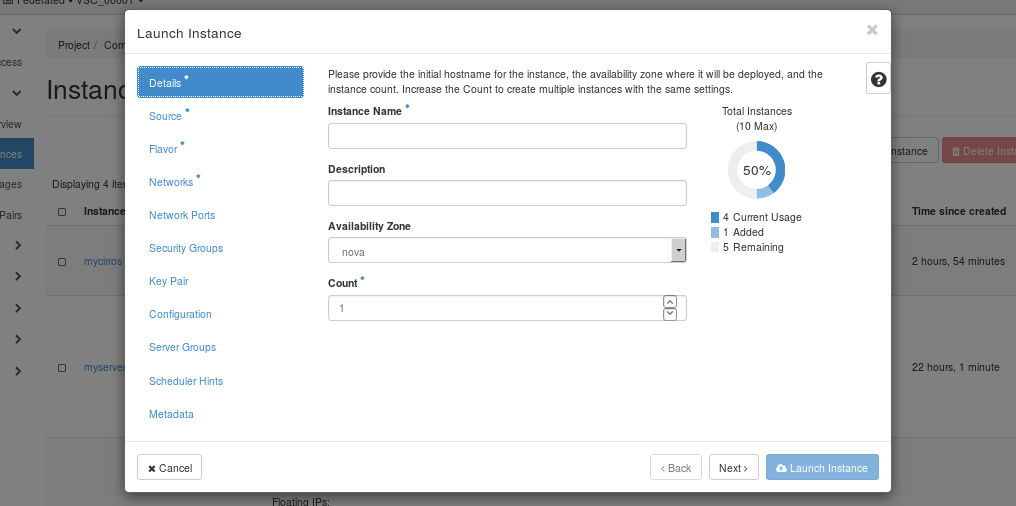
\includegraphics[scale=0.5]{img/tab-compute-instances-launch.png}
\end{center}


\strong{Update an image}

Follow this procedure to update an existing image.

\begin{enumerate}
\def\labelenumi{\arabic{enumi}.}
\item
  \begin{quote}
  Log in to the dashboard.
  \end{quote}
\item
  \begin{quote}
  Select the appropriate project from the drop down menu at the top
  left.
  \end{quote}
\item
  \begin{quote}
  Select the image that you want to edit.
  \end{quote}
\item
  \begin{quote}
  In the Actions column, click the menu button and then select Edit
  Image from the list.
  \end{quote}
\item
  \begin{quote}
  In the Edit Image dialog box, you can perform various actions. For
  example:
  \end{quote}

  \begin{itemize}
  \item
    \begin{quote}
    Change the name of the image.
    \end{quote}
  \item
    \begin{quote}
    Change the description of the image.
    \end{quote}
  \item
    \begin{quote}
    Change the format of the image.
    \end{quote}
  \item
    \begin{quote}
    Change the minimum disk of the image.
    \end{quote}
  \item
    \begin{quote}
    Change the minimum RAM of the image.
    \end{quote}
  \item
    \begin{quote}
    Select the Public button to make the image public.
    \end{quote}
  \item
    \begin{quote}
    Clear the Private button to make the image private.
    \end{quote}
  \item
    \begin{quote}
    Change the metadata of the image.
    \end{quote}
  \end{itemize}
\item
  \begin{quote}
  Click Edit Image.
  \end{quote}
\end{enumerate}
